\chapter{Clustering}

In the field of clustering analysis, there is no strict definition for cluster itself. That may be one reason why there is such a vast amount of clustering algorithms; many authors such as \citet{estivill2002so} discuss this topic.  However, the one think in common that we can find among all the algorithms is a work with a group of data objects.

Suppose data $\mathcal{D}$ given as a $n$ $d$-dimensional vectors $(x_1,\dots,x_d) \subset \R_d$  -- objects; each element of a vector describes specific object property. Two objects are similar if values of their respective properties are alike. Then, clustering analysis can be defined as a form of grouping objects into subsets of $\mathbf{D}$ while maximizing inter-set object similarity and minimizing intra-set object similarity.

\section{Clustering models}

Concrete variations of clustering analysis are defined by a clustering model. They are divided into several sections.

\subsection{Centroid-based model}

\emph{Centroid-based clustering model} represents clusters only by a central vector --- \emph{centroid} (see def. \ref{def01:centr}) --- which is not necessarily a member of a working set. Many implementations of this model need the number of required centroids in advance. We define the following optimalization problem for this kinds of algorithms. 

\begin{problem}
	Having a distance function $d$, find $k$ centroids $C_1,\dots,C_k$ from the domain of the dataset $\mathcal{D}$ such that the sum \ref{eq01:sum}
	is minimized.
\end{problem}

\begin{equation}\label{eq01:sum}
	\sum_o^{\mathcal{D}} \min_{i=1\dots k}d(o,C_i)
\end{equation}

This problem is uneasy to solve due to its exponential complexity. Hence, many approximation algorithms emerged. 

\begin{defn}
	Suppose a cluster $\mathcal{C} \subset \R^d$. We define the \emph{centroid} $c \in \R^d$ of the cluster $\mathcal{C}$ as the average of all points $o \in \mathcal{C}$. 
	\label{def01:centr}
\end{defn}

\subsubsection{k-means}

The most common implementation of centroid-based clustering is \emph{k-means}. Its algorithm can be expressed in a few simple steps (see \ref{alg01:kmeans}).

\begin{algorithm}
	\caption{$k$-means clustering}
	\label{alg01:kmeans}
	\begin{algorithmic}[1]
		\Procedure{$k$-means}{$k\in\R$, $\mathcal{D} \subset \R^d$, $d \in \R^d \times \R^d \to \R$}
		\State $\mathcal{C} \gets$ first $k$ objects from  $\mathcal{D}$ \Comment{select initial centroids}
		\Repeat
			\For{$i \in \{1\dots k\}$}
				\State $K_i \gets \{\}$\Comment{create empty clusters}
			\EndFor
			\ForAll{$o \in \mathcal{D}$}
				\State $i' \gets$ index of the closest centroid $c_i \in \mathcal{C}$ to $o$; $d(o,c_i)$ is minimal
				\State $K_{i'} \gets K_{i'} \cup o$ \Comment{assign objects to clusters}
			\EndFor
			\For{$i \in \{1\dots k\}$}
				\State $c'_i \gets$ centroid of $K_i$ \Comment{compute new centroids}
			\EndFor
			\State $\mathcal{C}' \gets \{c'_1,\dots,c'_k\}$
			\State swap $\mathcal{C}$ and $\mathcal{C}'$
		\Until{$\mathcal{C} = \mathcal{C}^\prime$}
		\State \textbf{return} $\mathcal{C}$
		\EndProcedure
	\end{algorithmic}
\end{algorithm}


The algorithm divides data into $k$ clusters (hence, \emph{k}-means) in a iterative manner. Before the first iteration, initial $k$ central vectors are selected from the dataset. Each iteration, dataset objects are grouped into clusters according to the closest centroid. After that, new centroids are then computed from new clusters. Next iteration follows until centroids does not change or predefined number of iterations is reached. 

The advantage of this algorithm is the fact that it is easily comprehensible; hence can sustain for large variety of datasets. Another think is that it is said to be the speediest centroid-based algorithm. However, the disadvantages are inability to deal with the noise in a dataset and clusters of non-convex shape~\cite{uppada2014centroid}.
  

\subsection{Hierarchical model}

In \emph{Hierarchical clustering model}, objects are \emph{connected} together forming tree-like structure. In contrast with the aim of centroid-based model returning only $k$ centroids, hierarchical clustering algorithms capture whole connecting process. The algorithm starts with all objects from a dataset being initial clusters. Each iteration, two clusters are connected creating a new one finishing with one all-inclusive cluster. Commonly, this algorithms represent the connecting process as an ordered list of pairs --- connected clusters~\cite{karypis1999chameleon}.

The above described approach of a hierarchical algorith is called \emph{agglomerative} approach. The algorithm begins with each object representing a cluster on its own. Then, in a bottom-up fashion clusters are successively connected into the only cluster. The other option is \emph{divisive approach}. Beginning with a single all-inclusive cluster it is divided into sub-clusters until single objects remain~\cite{rokach2005clustering}. 

The result of hierarchical clustering can be viewed in a \emph{dendrogram} (see fig. \ref{fig01:dendro}). The x-axis states the distance of connected clusters. The y-axix shows the objects from a dataset.

\begin{figure}\centering
	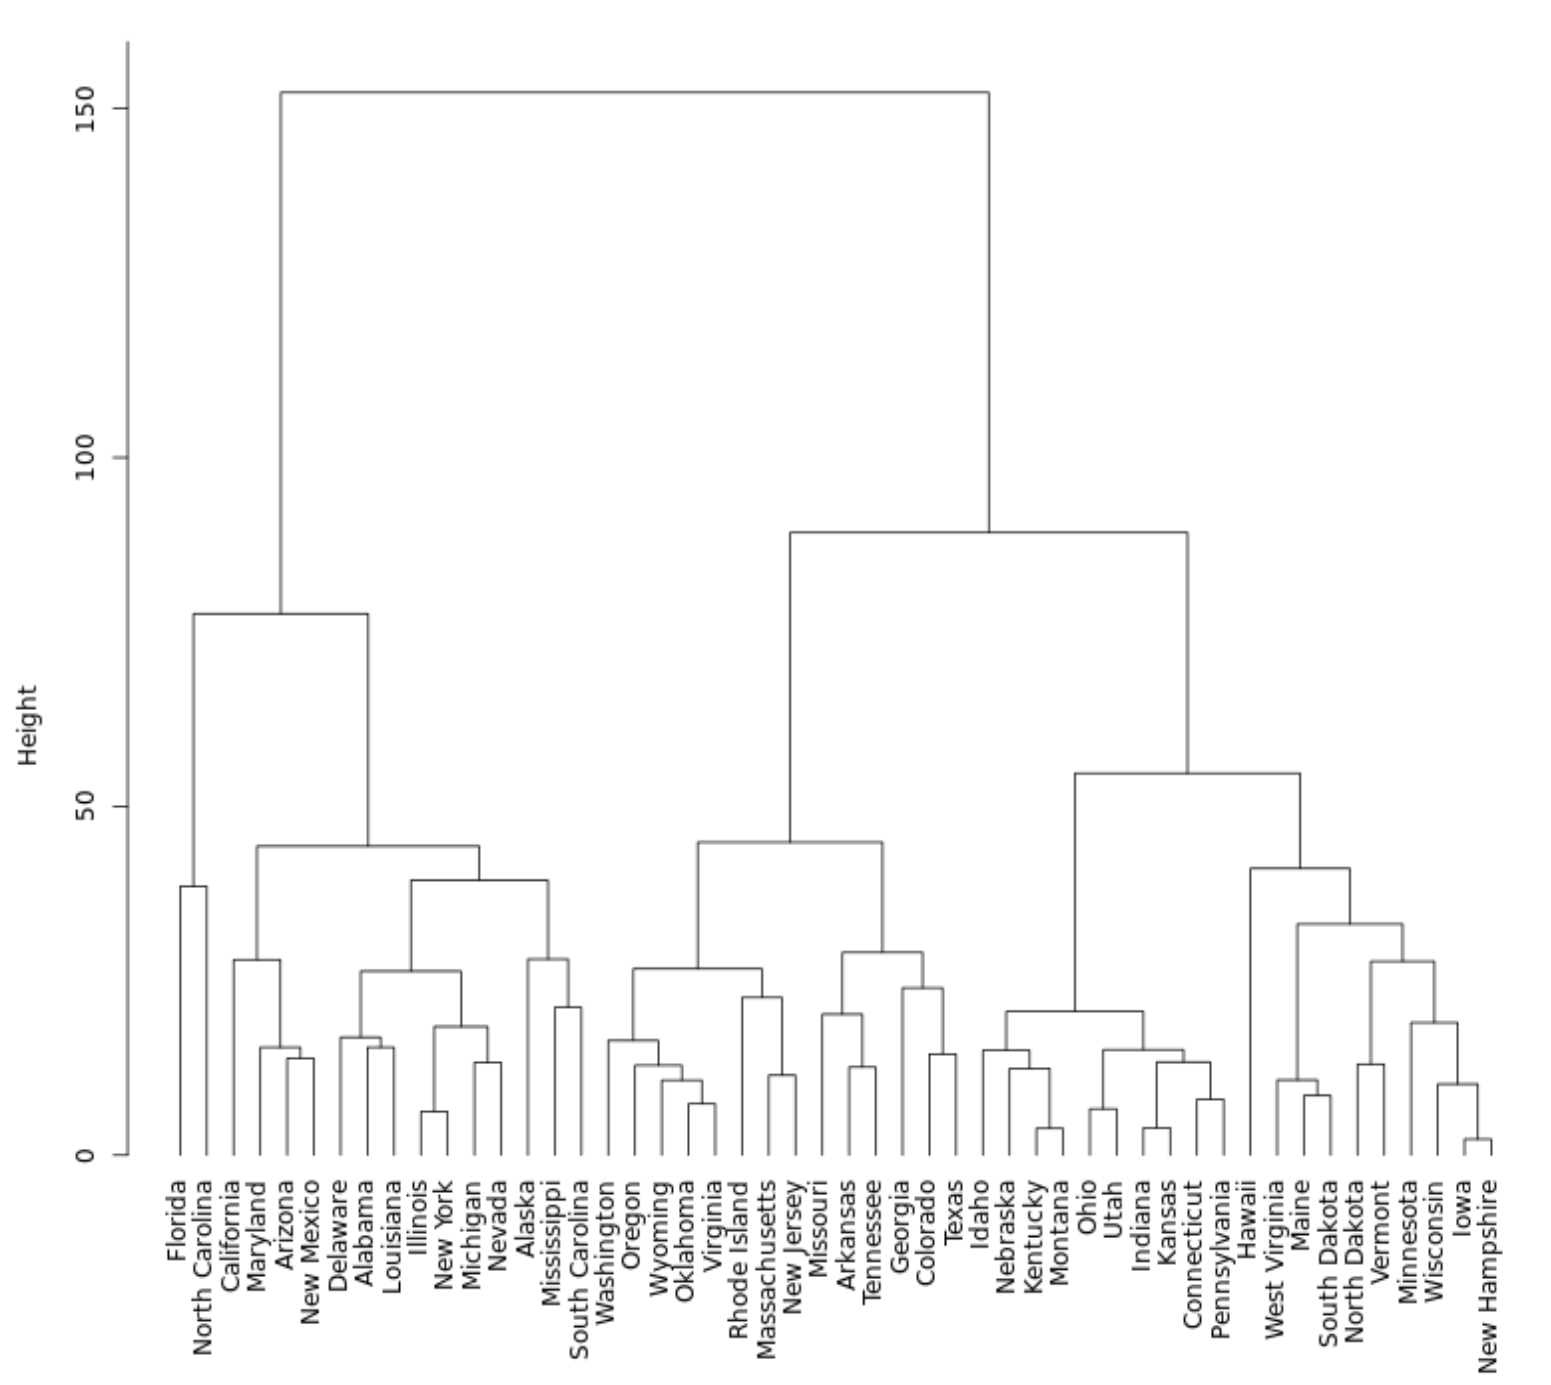
\includegraphics[width=\linewidth]{img/dendro}
	\caption{An example of dendrogram. placeholder }
	\label{fig01:dendro}
\end{figure}

To know which two clusters are connected (or respectively, how a cluster is divided into two), algorithms use a \emph{measure of a dissimilarity} between clusters.  
Hierarchical model distinguishes various kind of algorithms based on the choice of this measure. Commonly, the computation is dependent on the two factors; \emph{distance function} and \emph{linkage criterion}. 

\subsubsection{Distance functions}

\emph{Distance function} is used on objects of a dataset to express how far they are from each other in the observed domain. Supposing objects are represented as vectors $v_i \in \R_d$, variations of \emph{Minkowski distance formula} (see \ref{eq01:mink}) are the most commonly used.
This variations are \emph{Manhattan distance} ($p=1$), \emph{Euclidean distance} ($p=2$) and \emph{Chebyshev distance} ($p \to \infty$) (see table \ref{tab01:mink}).

It is obvious that the choice of a distance function can influence the result of a clustering. Hence, it should be chosen with respect to the properties of a provided dataset. \citet{aggarwal2001surprising} show the qualitative behavior of different distance functions in the $k$-means algorithm.  

\begin{equation}\label{eq01:mink}
||a-b||_p = (\sum_{i=1...d}|a_i-b_i|^p)^{\frac{1}{p}}
\end{equation}

\begin{table}
	\centering
	\begin{tabular}{ll}
		\toprule
		Manhattan & $||a-b||_1 = \sum_{i=1...d}|a_i-b_i|$          \\
		Euclidean & $||a-b||_2 = \sqrt{\sum_{i=1...d}(a_i-b_i)^2}$ \\
		Chebyshev & $||a-b||_\infty = \max_{i=1\dots d}|a_i-b_i|$  \\ \bottomrule
	\end{tabular}
	\caption{Variations of Minkowski distance formula.}
	\label{tab01:mink}
\end{table}

\subsubsection{Linkage criteria}

As the reader may have already discovered, one particular problem arises. The hierarchical algorithm can not compute proximity of two clusters only using distance function as it is the function of \emph{dataset objects} Hence, we define a function of \emph{object clusters} to complete the process of measuring dissimilarity -- \emph{linkage criterion}. Supposing clusters $A$ and $B$ as sets of dataset objects and distance function $d$, wer define following \emph{linkage criteria}~\cite{yim2015hierarchical}:

\begin{description}
	\item[Single linkage] -- Also referred to as minimum method, \emph{single linkage criterion} computes distance between $A$ and $B$ as the minimum distance between any pair $(a,b) \in A\times B$ (see  \ref{eq01:single_link}).
	\begin{equation}\label{eq01:single_link}
	\min\{d(a,b) : a \in A, b \in B\}
	\end{equation}
	
	The major drawback this criterion suffers is \emph{cluster chaining}. Such two clusters can be connected that they do not share any other pair of close proximity objects than the one that determined the connection. This produces long thin clusters with great distance between some objects.
	
	\item[Complete linkage] -- Also referred to as maximum method, \emph{complete linkage criterion} is similar to the single linkage criterion. But as opposed to to finding minimum, this criterion uses the maximum of object pairs in computing cluster dissimilarity (see \ref{eq01:complete_link}). 
	\begin{equation}\label{eq01:complete_link}
	\max\{d(a,b) : a \in A, b \in B\}
	\end{equation}
	
	The criterion suffers from its simplicity as well as the single linkage. But instead of naively connecting dissmimilar clusters, here simmilar clusters are not connected in some cases. Having all two clusters' objects in close proximity to each other but one object being rather far from the others, the criterion will not link the clusters as the maximum distance deteriorates the rest.
	
	\item[Centroid linkage] -- \emph{Centroid linkage criterion} tries to solve problems of criteria above by measuring the distance between the centroids of clusters. It introduces a form of an average into the computation; the think that criteria above lack.
\end{description}

A choice of a linkage criterion in hierarchical clustering algorithm is vital. As stated above, it can change the course of clustering in a great manner. Chosen improperly, it can have disastrous effect on the resulting solution.

\begin{figure}\centering
	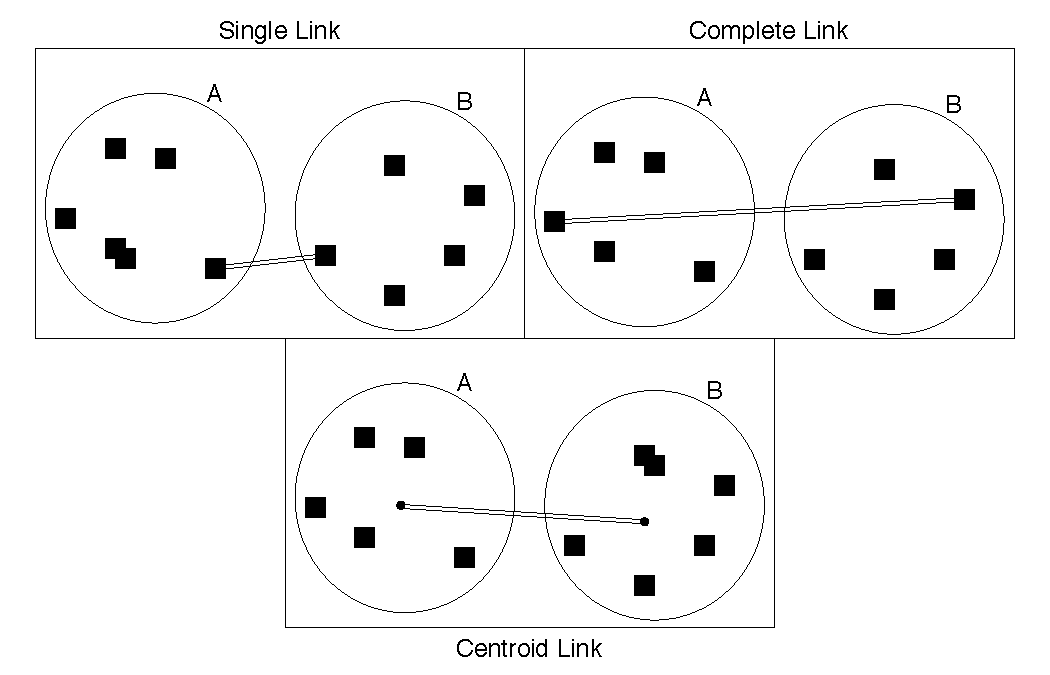
\includegraphics[width=10cm]{img/linkage_criteria}
	\caption{Example of linkage criteria. The double line represents the distance between clusters A and B according to the respective criterion.}
	\label{fig01:link}
\end{figure}

\section{Mahalanobis-based clustering}

To produce more meaningful results, hierarchical clustering algorithms have branched into many variations each focusing on a specific dataset types. \emph{Ma\-ha\-la\-no\-bis-based hierarchical clustering analysis} (MHCA) focuses on datasets that create clusters of ellipsoid shapes. This datasets are common products during natural measurements of cell cytometry data in bio-informatics.

\subsection{Mahalanobis distance}

The significant part of this clustering variation is the measure of cluster dissimilarity. It is based on the \emph{Mahalanobis distance} \cite{mahalanobis1936generalized} (see def. \ref{def01:maha}), a distance between a point and a set of points (in our case a cluster). If points in the set are strongly correlated in some axis then points laying on the axis are closer to the set than points that are not; even if their euclidian distance to the center of the set is closer.

\begin{defn}
	Suppose we have a cluster of $d$-dimensional points $\mathcal{C} \subset \R^d$. We define \emph{the random vector of a cluster} $\mathbf{v}$ as a $d$-element vector; the $i$-th element being a discrete random variable with equal probability values $\{o_i:o\in \mathcal{C}\}$
\end{defn}

\begin{defn}
	Suppose we have a cluster of $d$-dimensional points $\mathcal{C} \subset \R^d$, the centroid $c$ of $\mathcal{C}$ and covariance matrix $\mathcal{S}$ from the random vector $\mathbf{v}$ of the cluster $\mathcal{C}$. \emph{Mahalanobis distance} between $u \in \R^d$ and $\mathcal{C}$ is defined by the equation \ref{eq01:maha}.
	\begin{equation}\label{eq01:maha}
	d_M(u,\mathcal{C}) = \sqrt{(u-c)^TS^{-1}(u-c)}
	\end{equation}
	\label{def01:maha}
\end{defn}


With \emph{Mahalanobis distance}, we are able to compute a point-cluster proximity. To fully incorporate the distance in a hierarchical algorithm, we need to find a method how to measure cluster-cluster proximity. There are two options how to achieve this. 

First, we can choose a path of the single and complete linkage criterion; hence, all points in cluster contribute to the measure. We achieve this with \emph{Full Mahalanobis distance} (FMD) (see def. \ref{def01:fmd}).
The second option is similar to the centroid linkage as only the centroid of a cluster occurs in the computing. We define this as a \emph{Centroid Mahalanobis distance} (CMD) (see def. \ref{def01:cmd}).      

To easily imagine the measure, suppose we have two elliptic clusters. The algorithm favors such clusters that their ellipsis are alongside rather than in a prolongation of one another \cite{dagnelie1991using} (see fig. \ref{fig01:ellipses}). Only when the cluster objects are uncorrelated, this measure of dissimilarity is equal to the euclidean distance with an according linkage.

\begin{figure}\centering
	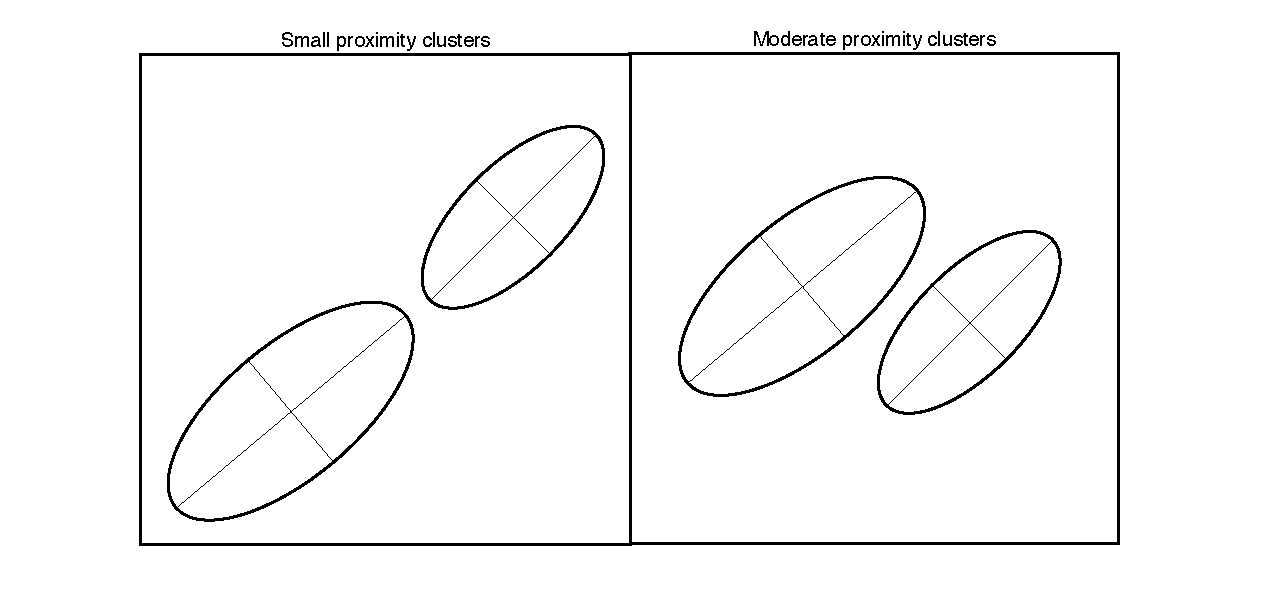
\includegraphics[width=10cm]{img/ellipses}
	\caption{Example of cluster dissimilarity in Mahalanobis-based hierarchical clustering.}
	\label{fig01:ellipses}
\end{figure}

\begin{defn}
	Suppose we have clusters $\mathcal{C}$ and $\mathcal{C}'$. We define the \emph{Full Mahalanobis distance} between clusters $\mathcal{C}$ and $\mathcal{C}'$ as an average of the mahalanobis distances between all objects $o \in \mathcal{C}$ and $\mathcal{C}'$ (see \ref{eq01:fmd}).
	\begin{equation}\label{eq01:fmd}
	d_{FM}(\mathcal{C},\mathcal{C}') =\frac{1}{|\mathcal{C}|}\sum_{o\in\mathcal{C}}{d_M(o,\mathcal{C}')}
	\end{equation}
	\label{def01:fmd}
\end{defn}

\begin{defn}
	Suppose we have a clusters $\mathcal{C}$ with its centroid $c$ and a cluster $\mathcal{C}'$. We define the \emph{Centroid Mahalanobis distance} between clusters $\mathcal{C}$ and $\mathcal{C}'$ as the mahalanobis distance between $c$ and $\mathcal{C}'$ (see \ref{eq01:cmd}).
	\begin{equation}\label{eq01:cmd}
	d_{CM}(\mathcal{C},\mathcal{C}')=d_M(c,\mathcal{C}')
	\end{equation}
	\label{def01:cmd}
\end{defn}


The pros and cons between FMD and CMD are trivial. Due to the full point contribution, FMC can produce more precise measure than its counterpart. On the other hand, CMD compensates is with the much needed time complexity. The current thesis will analyze the impact of both the methods in the following chapters.

\vspace{0.5cm}

To make use of this mahalanobis distance variants in MHCA implementations, we require distance funtion to be \emph{symmetric}. By its nature mahalanobis distance is not a symmetric funtion. However, we easily achieve this attribute with the \emph{Generalized distance} (see def. \ref{def01:gene}).

\begin{defn}
	Suppose we have clusters $\mathcal{C}$, $\mathcal{C}'$ and a variant of mahalanobis distance~$d$ (either FMD or CMD). We define the \emph{Generalized distance} between clusters $\mathcal{C}$ and $\mathcal{C}'$ as an average distance between $\mathcal{C}$, $\mathcal{C}'$ and $\mathcal{C}'$, $\mathcal{C}$ (see \ref{eq01:gene}).
	\begin{equation}\label{eq01:gene}
	d_G(\mathcal{C},\mathcal{C}') = \frac{d(\mathcal{C},\mathcal{C}')+d(\mathcal{C}',\mathcal{C})}{2}
	\end{equation}
	\label{def01:gene}
\end{defn}  


\subsection{Algorithm optimizations}

In early stages of MHCA it is sub-optimal to use full \emph{generalized distance}. It is due to the fact that clusters with one to few points does not form computable ellipsoids; in other words, Mahalanobis distance equation would produce distorted results. 

To solve this problem, we used the variant of euclidean distance with centroid linkage on clusters with their size under specified threshold. The value of the threshold is proportional to the size of a dataset varying at about 0.1\% of the dataset size \cite{fivser2012detection}. Hence, to implement this optimization we defined \emph{Altered general distance} (see def. \ref{def01:alt}).

\begin{defn}
	Suppose a threshold $T_M$, a cluster $\mathcal{C}$ with its centroid $c$ and a cluster $\mathcal{C}'$ with its centroid $c'$ and a variant of mahalanobis distance $d$. We define \emph{Altered general distance} by equation \ref{eq01:alt}:
	\begin{equation}
	d_A(\mathcal{C},\mathcal{C}')=
	\begin{cases}
	d_G(\mathcal{C}, \mathcal{C}'), & \text{if $|\mathcal{C}|\ge T_M$ and $|\mathcal{C}'|\ge T_M$},\\
	\dfrac{d(\mathcal{C}, \mathcal{C}')+||c-c'||_2}{2}, & \text{if $|\mathcal{C}| < T_M$ and $|\mathcal{C}'|\ge T_M$},\\
	\dfrac{||c-c'||_2+d(\mathcal{C}', \mathcal{C})}{2}, & \text{if $|\mathcal{C}|\ge T_M$ and $|\mathcal{C}'|< T_M$},\\
	||c-c'||_2, & \text{if $|\mathcal{C}|< T_M$ and $|\mathcal{C}'|< T_M$}.\\
	\end{cases}
	\label{eq01:alt}
	\end{equation}
	\label{def01:alt}
\end{defn}



\section{Algorithm complexity}

The common problem in clustering algorithms is their \emph{time complexity}. In hierarchical clustering algorithms, we trivially achieve time complexity of $O(n^3)$ using $O(n^2)$ space. This restricts the use of the algorithms to dataset sizes varying between $10^3$ and $10^5$ points. Be aware that this restrictions is present not only due to the time complexity; the current computers can only with great difficulties store $10^6$ data points with the mentioned \emph{space complexity}.

Let us elaborate more about the space and time complexity of the hierarchical clustering analysis (HCA) algorithms. \citet{day1984efficient} describes three implementations of HCA. In this thesis, we employ them in the manner of further research and describe them with emphases on the algorithm complexity:

\begin{description}
	\item[HCA with the dissmilarity matrix] -- The first and the most trivial implementation uses the \emph{dissimilarity matrix} $M$ (see def. \ref{def01:dismat}). Unless there remains only one cluster, the algorithm searches $M$ for the closest pair of clusters, stores the pair and updates $M$ (see alg. \ref{alg01:dismat}).
	
	\begin{defn}
		Suppose a dataset $\mathcal{D}$ divided into clusters $C_1,\dots,C_m$ and a function $d$ as a measure of dissimilarity. Then, the \emph{dissimilarity matrix} $M$ is $m\times m$ matrix where $M_{ij} = d(C_i,C_j)$.
		\label{def01:dismat}
	\end{defn}
	
	\begin{algorithm}
		\caption{HCA with dissimilarity matrix}
		\label{alg01:dismat}
		\begin{algorithmic}[1]
			\Procedure{dismat}{$\mathcal{D} \subset \R^d$}
			\State initialize the dissimilarity matrix $M$
			\For{$k=|\mathcal{D}|$ \textbf{downto} $1$}
			\State search $M$ for the closest pair $(i,j)$ \Comment{time: $O(k^2)$}
			\State store cluster pair $(i,j)$ into the merge list \Comment{time: $O(1)$}
			\State update $M$ \Comment{time: $O(k)$}
			\EndFor
			\State \textbf{return} list of merged clusters
			\EndProcedure
		\end{algorithmic}
	\end{algorithm}

	The main cycle in line $3$ repeats $n = |\mathbb{D}|$ times; each time the number of clusters being reduced by 1. The search in line $4$ is bounded by $O(n^2)$ time, having its peak in the first iteration when $k=n$. The update in line $6$ is required to reflect deletion of clusters $i$ and $j$ and addition of the new one. Hence, it needs to perform $k$ new dissimilarity measures for the new cluster (bounded by $O(n)$ during the first iteration as well). As there are $n$ iterations performed, this results in the overall time complexity of $O(n^3)$. 
	
	The space required to store $M$ is in $O(n^2)$. As there is no other non-trivial requirement, space complexity is $O(n^2)$. 
	\begin{rem}
		However, there is no need to store the matrix at all. We can choose to measure cluster dissimilarity \emph{in-place}. Line $6$ would become redundant and the time complexity of line $4$ would increase by a constant multiplicative factor; hence, time complexity remains the same while the space complexity becomes $O(n)$.
	\end{rem}
	

	\item[HCA with the nearest neighbor array] -- This algorithm introduces the array of the nearest neighbour (see def. \ref{def01:neigh}). Instead of the dissimilarity matrix, each cluster is assigned the index of the closest neighboring cluster (see alg. \ref{alg01:neigh}).
	
	\begin{defn}
		Suppose a dataset $\mathcal{D}$ divided into clusters $C_1,\dots,C_m$ and a function $d$ as a measure of dissimilarity. Then, the \emph{nearest neighbor array} $N$ is $m$-element array of indices $\{1,\dots,m\}$ where each element $N_i$ satisfies the equation \ref{eq01:neigh}.
		\begin{equation}
			d(C_i,C_{N_i}) = \min\{d(C_i,C_j) : j \in \{1,\dots,m\} \setminus \{i\}\}
			\label{eq01:neigh}
		\end{equation}
		
		\label{def01:neigh}
	\end{defn}
	
	\begin{algorithm}
		\caption{HCA with the nearest neighbor array}
		\label{alg01:neigh}
		\begin{algorithmic}[1]
			\Procedure{neighbor}{$\mathcal{D} \subset \R^d$}
			\State initialize $N$
			\For{$k=|\mathcal{D}|$ \textbf{downto} $1$}
			\State search $N$ for the closest pair $(i,j)$ \Comment{time: $O(k)$}
			\State store cluster pair $(i,j)$ into the merge list \Comment{time: $O(1)$}
			\State update $N$ \Comment{time: $O(k^2)$}
			\EndFor
			\State \textbf{return} list of merged clusters
			\EndProcedure
		\end{algorithmic}
	\end{algorithm}
	
	Compared to the alg. \ref{alg01:dismat}, this algorithm trades the expensive \emph{closest pair search} with the expensive \emph{structure update}:
	
	 In line $4$, each closest pair search can be performed in $O(n)$ time as the array length does not exceeds $n$ elements. However in line $6$, the worst case update of $N$ happens when every cluster is in the closest neighborhood with the clusters that are being merged; the clusters of indices $i$ and $j$. In this case, the whole array has to be recomputed, which corresponds to the computation of the whole dissimilarity matrix. Hence, the time complexity for this step is $O(n^2)$. The overall time complexity is $O(n^3)$. The space complexity is $O(n)$ as $N$ does not have more than linear space requirements.
	 
	 \begin{rem}
	 	Despite equal time complexities, this algorithm may outperform the previous one as in the majority of situations the update step in line $6$ does not require the whole array to be recomputed. Moreover, if the number of elements to be updated will be constant each iteration, the overall algorithm time complexity may be $O(n^2)$. 
	 \end{rem}
	 
	 \item[HCA with priority queues] -- This algorithm takes advantage of the previous one employing the fast search and combines it with the fast update using \emph{priority queues} (see alg. \ref{alg01:queue}).
	 
	 \begin{algorithm}
	 	\caption{HCA with priority queues}
	 	\label{alg01:queue}
	 	\begin{algorithmic}[1]
	 		\Procedure{queues}{$\mathcal{D} \subset \R^d$}
	 		\ForAll{$o \in \mathcal{D}$}
	 		\State initialize a priority queue from $\mathcal{D} \setminus \{o\}$
	 		\EndFor
	 		\For{$k=|\mathcal{D}|$ \textbf{downto} $1$}
	 		\State search $k$ queues for the closest pair $(i,j)$ \Comment{time: $O(k)$}
	 		\State store cluster pair $(i,j)$ into the merge list \Comment{time: $O(1)$}
	 		\State update $k$ priority queues \Comment{time: $O(k\log{k})$}
	 		\EndFor
	 		\State \textbf{return} list of merged clusters
	 		\EndProcedure
	 	\end{algorithmic}
	 \end{algorithm}
 
 	The priority label of a queued element is the dissimilarity measure. 
 	
 	As operation for retrieving a minimum in a priority queue has $O(1)$ time complexity, the search step in line $4$ takes $O(k)$ time (bounded by $O(n)$ during the first iteration). Next in line $6$, we need one insert and two delete operations (corresponding to deleting two merged clusters and inserting one new). As these operations require $O(\log{n})$ time, we can update $n$ queues in $O(n\log{n})$ time.
 	
 	To sum up, the overall time complexity is $O(n^2\log{n})$. The space complexity is back to $O(n^2)$ due to the linear space requirements of queue.
 	
 	\begin{rem}
 		Note that this is the only algorithm from the three described that unavoidably requires quadratic space. This may lead to the further restrictions of its usage having large datasets.
 	\end{rem}

\end{description}

\subsubsection{Example}

To fully show the algorithm complexity downside, we measured R language library function \texttt{hclust}; the frequenly used implementation of HCA. It computes centroid linkage with euclidean distance and uses dissimilarity matrix. 

Fig. \ref{fig01:hclust} shows above stated polynomial time complexity of the implementation. Moreover, it halted at a dataset size of $47 000$ as the testing machine \footnote{Intel Core i9-8950HK, 32GB RAM} ran out of memory.

In conclusion, we can see that the space complexity of HCA can be more restrictive in the means of overall algorithm usability than its time complexity. It can be easily solved by removing high space complexity structures (such as a dissimilarity matrix) for the price of lower speed while retaining the same asymptotic time complexity.

\begin{figure}\centering
	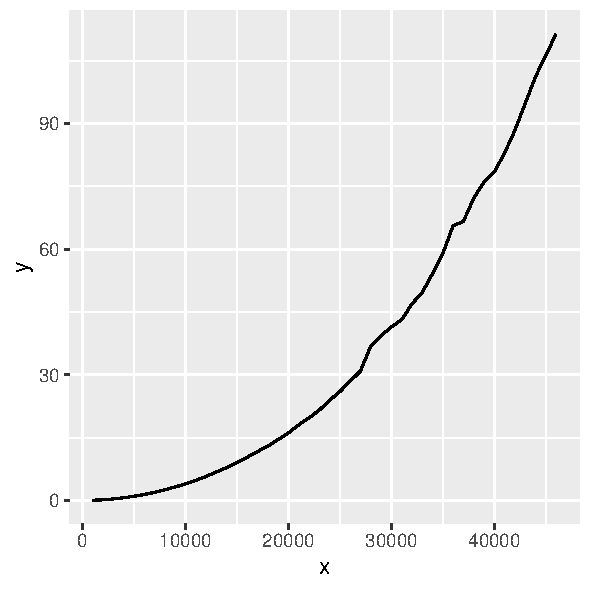
\includegraphics[width=10cm]{img/hclust}
	\caption{Time complexity of \texttt{hclust} according to the size of a dataset.}
	\label{fig01:hclust}
\end{figure}
